\documentclass[12pt]{article}
\usepackage[margin=0.8in]{geometry}
\usepackage{amsmath}
\usepackage{amssymb}
\usepackage{xcolor}
\usepackage{tikz}
\usepackage{enumitem}

\title{\LARGE CES Utility: What Changes as $s$ Changes?\\Q1(b) Explained}
\author{ECO 310}
\date{}

\setlength{\parskip}{0.5em}

\begin{document}

\maketitle

\section*{The Big Confusion}

When Q1(b) asks "what happens as $s \to 0$", students often think the budget line changes.

\begin{center}
\colorbox{red!20}{
\Large
\textbf{THE BUDGET LINE DOES NOT CHANGE!}
}
\end{center}

\vspace{1em}

The budget line is:
$$p_1 x_1 + p_2 x_2 = m$$

It only depends on \textbf{prices and income}, which are fixed in Q1(b).

\section*{What DOES Change?}

\begin{center}
\colorbox{green!20}{
\Large
\textbf{Your indifference curves change shape!}
}
\end{center}

The CES utility function is:
$$u(x_1, x_2) = (x_1^s + x_2^s)^{1/s}$$

As $s$ changes, the shape of your indifference curves changes, which makes you choose \textbf{different points on the same budget line}.

\section*{Visual Explanation}

Imagine a fixed budget line (same prices, same income):

\begin{center}
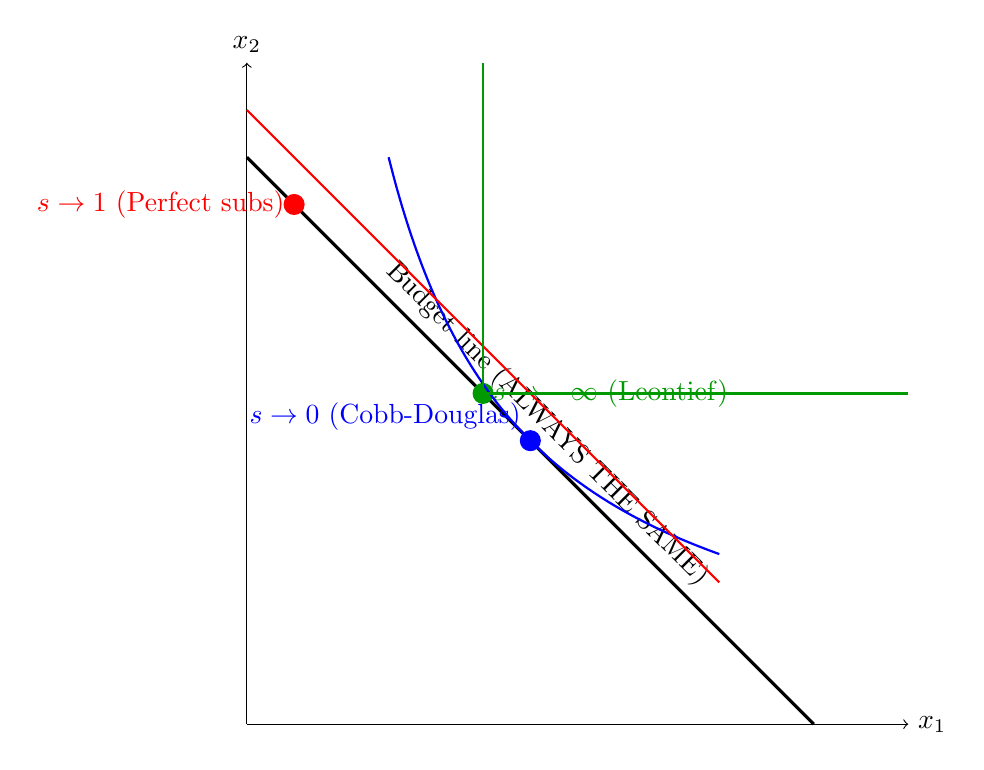
\begin{tikzpicture}[scale=1.2]
% Same budget line for all
\draw[very thick, black] (0, 6) -- (6, 0);
\node[black, above, rotate=-45] at (3, 3) {Budget line (ALWAYS THE SAME)};

% Axes
\draw[->] (0,0) -- (7,0) node[right] {$x_1$};
\draw[->] (0,0) -- (0,7) node[above] {$x_2$};

% Three different optimal points
\filldraw[blue] (3, 3) circle (3pt) node[above left] {$s \to 0$ (Cobb-Douglas)};
\filldraw[red] (0.5, 5.5) circle (3pt) node[left] {$s \to 1$ (Perfect subs)};
\filldraw[green!60!black] (2.5, 3.5) circle (3pt) node[right] {$s \to -\infty$ (Leontief)};

% Indifference curves (sketched)
% Cobb-Douglas: smooth curve
\draw[blue, thick, domain=1.5:5, smooth, samples=50] plot (\x, {9/\x});

% Perfect substitutes: straight line
\draw[red, thick] (0, 6.5) -- (5, 1.5);

% Leontief: L-shape
\draw[green!60!black, thick] (2.5, 7) -- (2.5, 3.5) -- (7, 3.5);

\end{tikzpicture}
\end{center}

\textbf{Same budget line, different indifference curves, different optimal choices!}

\newpage

\section*{The Three Cases}

\subsection*{Case 1: $s \to 0$ (Cobb-Douglas)}

\textbf{Indifference curves:} Smooth, curved hyperbolas

\textbf{Demand functions approach:}
$$x_1^* = \frac{m}{2p_1}, \quad x_2^* = \frac{m}{2p_2}$$

\textbf{Interpretation:} You spend a constant fraction of income on each good (50\% on good 1, 50\% on good 2).

\textbf{On the budget line:} You choose an \textbf{interior point} where the IC is tangent to the budget line.

\begin{center}
\begin{tikzpicture}[scale=1.5]
\draw[->] (0,0) -- (5,0) node[right] {$x_1$};
\draw[->] (0,0) -- (0,5) node[above] {$x_2$};

% Budget line
\draw[thick, black] (0, 4) -- (4, 0) node[midway, below right] {Budget};

% Smooth IC
\draw[thick, blue, domain=1:3.5, smooth, samples=50] plot (\x, {4/\x});
\node[blue, right] at (3.5, 4/3.5) {IC};

% Tangency point
\filldraw[blue] (2, 2) circle (2pt) node[above right] {Optimal: $(2, 2)$};

% Tangent line
\draw[blue, dashed] (0.5, 3.5) -- (3.5, 0.5);

\end{tikzpicture}
\end{center}

\textbf{Key: Interior solution with tangency.}

\subsection*{Case 2: $s \to 1$ (Perfect Substitutes)}

\textbf{Indifference curves:} Straight lines with slope $= -1$

\textbf{Demand functions approach:}
$$\text{If } p_1 < p_2: \quad x_1^* = \frac{m}{p_1}, \, x_2^* = 0$$
$$\text{If } p_2 < p_1: \quad x_1^* = 0, \, x_2^* = \frac{m}{p_2}$$
$$\text{If } p_1 = p_2: \quad \text{Any bundle on the budget line}$$

\textbf{Interpretation:} Buy only the cheaper good (corner solution).

\textbf{On the budget line:} You choose a \textbf{corner point} (all of one good, none of the other).

\begin{center}
\begin{tikzpicture}[scale=1.5]
\draw[->] (0,0) -- (5,0) node[right] {$x_1$};
\draw[->] (0,0) -- (0,5) node[above] {$x_2$};

% Budget line (assume p1 < p2, so steeper)
\draw[thick, black] (0, 3) -- (4, 0) node[midway, above right] {Budget};

% Straight line ICs
\draw[thick, red] (0, 4.5) -- (3.5, 1);
\draw[thick, red] (0.5, 4.5) -- (4, 1.5);

% Corner solution
\filldraw[red] (4, 0) circle (2pt) node[below right] {Optimal: $(4, 0)$};

\node[red, above] at (2, 3) {IC};

\end{tikzpicture}
\end{center}

\textbf{Key: Corner solution - buy all of the cheaper good.}

\newpage

\subsection*{Case 3: $s \to -\infty$ (Perfect Complements / Leontief)}

\textbf{Indifference curves:} L-shaped with kink at $x_1 = x_2$

\textbf{Demand functions approach:}
$$x_1^* = \frac{m}{p_1 + p_2}, \quad x_2^* = \frac{m}{p_1 + p_2}$$

\textbf{Interpretation:} You consume goods in a fixed ratio (here, 1:1).

\textbf{On the budget line:} You choose the point where the \textbf{kink} of the IC touches the budget line.

\begin{center}
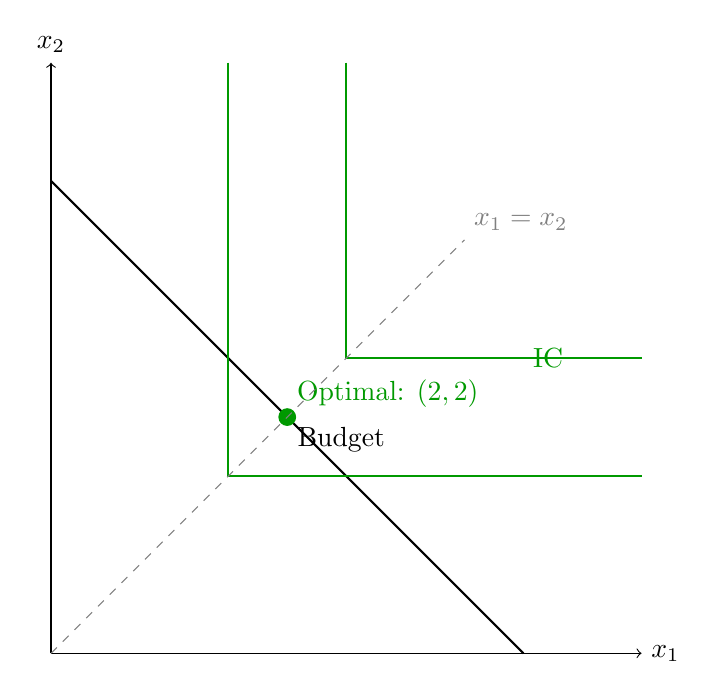
\begin{tikzpicture}[scale=1.5]
\draw[->] (0,0) -- (5,0) node[right] {$x_1$};
\draw[->] (0,0) -- (0,5) node[above] {$x_2$};

% Budget line
\draw[thick, black] (0, 4) -- (4, 0) node[midway, below right] {Budget};

% L-shaped ICs
\draw[thick, green!60!black] (1.5, 5) -- (1.5, 1.5) -- (5, 1.5);
\draw[thick, green!60!black] (2.5, 5) -- (2.5, 2.5) -- (5, 2.5);

% Optimal at kink
\filldraw[green!60!black] (2, 2) circle (2pt) node[above right] {Optimal: $(2, 2)$};

\node[green!60!black, right] at (4, 2.5) {IC};

% 45-degree line
\draw[dashed, gray] (0, 0) -- (3.5, 3.5) node[above right] {$x_1 = x_2$};

\end{tikzpicture}
\end{center}

\textbf{Key: Optimal at the kink - consume in fixed ratio.}

\section*{Summary Table}

\begin{center}
\begin{tabular}{|l|l|l|}
\hline
\textbf{As $s \to$} & \textbf{IC Shape} & \textbf{Optimal Point on Budget Line} \\
\hline
$0$ (Cobb-Douglas) & Smooth curves & Interior tangency \\
\hline
$1$ (Perfect subs) & Straight lines & Corner (buy cheaper good) \\
\hline
$-\infty$ (Leontief) & L-shaped & At the kink (fixed ratio) \\
\hline
\end{tabular}
\end{center}

\section*{The Key Insight for Q1(b)}

\begin{center}
\colorbox{yellow!30}{
\begin{minipage}{0.9\textwidth}
\textbf{What changes:} The shape of indifference curves

\textbf{What stays the same:} The budget line (same prices, same income)

\textbf{Result:} You choose different bundles on the same budget line
\end{minipage}
}
\end{center}

\newpage

\section*{How to Answer Q1(b)}

Q1(b) asks: "Show that as $s$ approaches certain values, your demand functions from (a) approach those for [Cobb-Douglas / Perfect Substitutes / Leontief]."

\subsection*{Step 1: Know the Target Demand Functions}

\textbf{Cobb-Douglas} $u = x_1^{1/2} x_2^{1/2}$:
$$x_1^* = \frac{m}{2p_1}, \quad x_2^* = \frac{m}{2p_2}$$

\textbf{Perfect Substitutes} $u = x_1 + x_2$:
$$\text{If } p_1 < p_2: \quad x_1^* = \frac{m}{p_1}, \quad x_2^* = 0$$
$$\text{If } p_2 < p_1: \quad x_1^* = 0, \quad x_2^* = \frac{m}{p_2}$$

\textbf{Leontief} $u = \min\{x_1, x_2\}$:
$$x_1^* = x_2^* = \frac{m}{p_1 + p_2}$$

\subsection*{Step 2: Take Your CES Demand from (a)}

From Q1(a), you should have derived:
$$x_1^* = \frac{m \cdot p_1^{\frac{s}{s-1}}}{p_1^{\frac{s}{s-1}} + p_2^{\frac{s}{s-1}}}$$

(or something similar depending on normalization)

\subsection*{Step 3: Take Limits}

\textbf{For $s \to 0$:}

Use L'Hospital's rule or the fact that as $s \to 0$:
$$p^{\frac{s}{s-1}} \to p^{-1}$$

So:
$$x_1^* \to \frac{m \cdot p_1^{-1}}{p_1^{-1} + p_2^{-1}} = \frac{m/p_1}{1/p_1 + 1/p_2} = \frac{m}{2p_1}$$

(assuming $p_1 = p_2$ for simplicity in the equal-weight case)

This matches Cobb-Douglas!

\textbf{For $s \to 1$:}

As $s \to 1$:
$$\frac{s}{s-1} \to \infty$$

So $p^{\frac{s}{s-1}}$ explodes for the larger $p$, meaning you spend all on the cheaper good.

This matches perfect substitutes!

\textbf{For $s \to -\infty$:}

The CES function approaches:
$$u = \min\{x_1, x_2\}$$

With kink condition $x_1 = x_2$ and budget constraint:
$$p_1 x_1 + p_2 x_2 = m \Rightarrow x_1(p_1 + p_2) = m \Rightarrow x_1 = \frac{m}{p_1 + p_2}$$

This matches Leontief!

\section*{What You Write on the Exam}

\textbf{Example for $s \to 0$:}

\textit{As $s \to 0$, the CES utility approaches Cobb-Douglas. Taking the limit of the demand function from (a):}

$$\lim_{s \to 0} x_1^* = \frac{m}{2p_1}$$

\textit{This matches the Cobb-Douglas demand where consumers spend a constant fraction of income on each good, independent of prices (in the equal-weight case).}

\textit{The budget line remains $p_1 x_1 + p_2 x_2 = m$, but the indifference curves become smooth hyperbolas, leading to an interior tangency solution.}

\vspace{2em}

\textbf{Key points to include:}
\begin{itemize}
    \item State what the limit is
    \item Show the demand approaches the target form
    \item Mention the shape of ICs (optional but helpful)
    \item Note the budget line stays the same (if asked)
\end{itemize}

\section*{Common Mistakes}

\begin{enumerate}[leftmargin=2cm, itemsep=1em]
    \item \textbf{Saying the budget line changes} - No! Only prices/income change the budget line.

    \item \textbf{Not taking the actual limit} - You need to show the algebra, not just say "it approaches."

    \item \textbf{Confusing $s$ values} - $s \to 0$ is Cobb-Douglas, $s \to 1$ is perfect subs, $s \to -\infty$ is Leontief.

    \item \textbf{Forgetting what changes vs what stays the same} - ICs change shape; budget line stays fixed.
\end{enumerate}

\end{document}
